\documentclass{article}

\usepackage[margin=1in]{geometry}
\usepackage{graphicx}
\usepackage{natbib}
\usepackage{amsmath,amssymb}
\usepackage{microtype}
\usepackage{hyperref}
\graphicspath{{./figures/}}

\begin{filecontents}{references.bib}
@article{chen2020simple,
  title={A Simple Framework for Contrastive Learning of Visual Representations},
  author={Chen, Ting and Kornblith, Simon and Norouzi, Mohammad and Hinton, Geoffrey},
  journal={ICML},
  year={2020}
}

@inproceedings{radford2021learning,
  title={Learning Transferable Visual Models From Natural Language Supervision},
  author={Radford, Alec and Kim, Jong Wook and Hallacy, Chris and et al.},
  booktitle={ICLR},
  year={2021}
}

@inproceedings{someOtherRef2021,
  title={Some Title},
  author={Doe, John and Roe, Richard},
  booktitle={Conference on Some Topic},
  year={2021}
}
\end{filecontents}

\bibliographystyle{plainnat}

\title{Challenges in Symbolic Consistency for Contrastive Pretraining}
\author{}
\date{}

\begin{document}

\maketitle

\begin{abstract}
We investigate the surprising pitfalls and partial successes of symbolic consistency under contrastive pretraining. Despite promising improvements, we highlight challenges that arise when applying these models to structured tasks in realistic settings, with potential negative downstream effects. 
\end{abstract}

\section{Introduction}
Deep learning methods have demonstrated strong performance on many tasks, yet symbolic or structured data domains introduce unexpected pitfalls. In contrastive learning approaches \citep{chen2020simple,radford2021learning}, even partial successes may mask real-world implementation challenges. We explore where these pitfalls arise and offer insights to guide future work.

\section{Related Work}
Prior work \citep{chen2020simple,radford2021learning} shows contrastive methods excel in natural image classification, but few studies examine symbolic tasks \citep{someOtherRef2021}. Our investigation highlights unique stability issues and domain-specific complexities often overlooked in previous literature.

\section{Method}
We adopt a contrastive pretraining strategy using standard image-text pairs. Our focus is on datasets that contain symbolic annotations. We freeze the main encoder and fine-tune a lightweight head for symbol classification. We varied several factors, including removing the projector, adjusting data augmentations, and skipping certain pretraining steps.

\section{Experiments}
Experiments were conducted on a small symbolic dataset with multiple derivations. We report cross-entropy loss curves and classification accuracy. Counterintuitively, removing the projector often caused degenerate representations that impaired downstream evaluation. This underscores the difficulty in ensuring consistent latent spaces.

\begin{figure}[t]
\centering
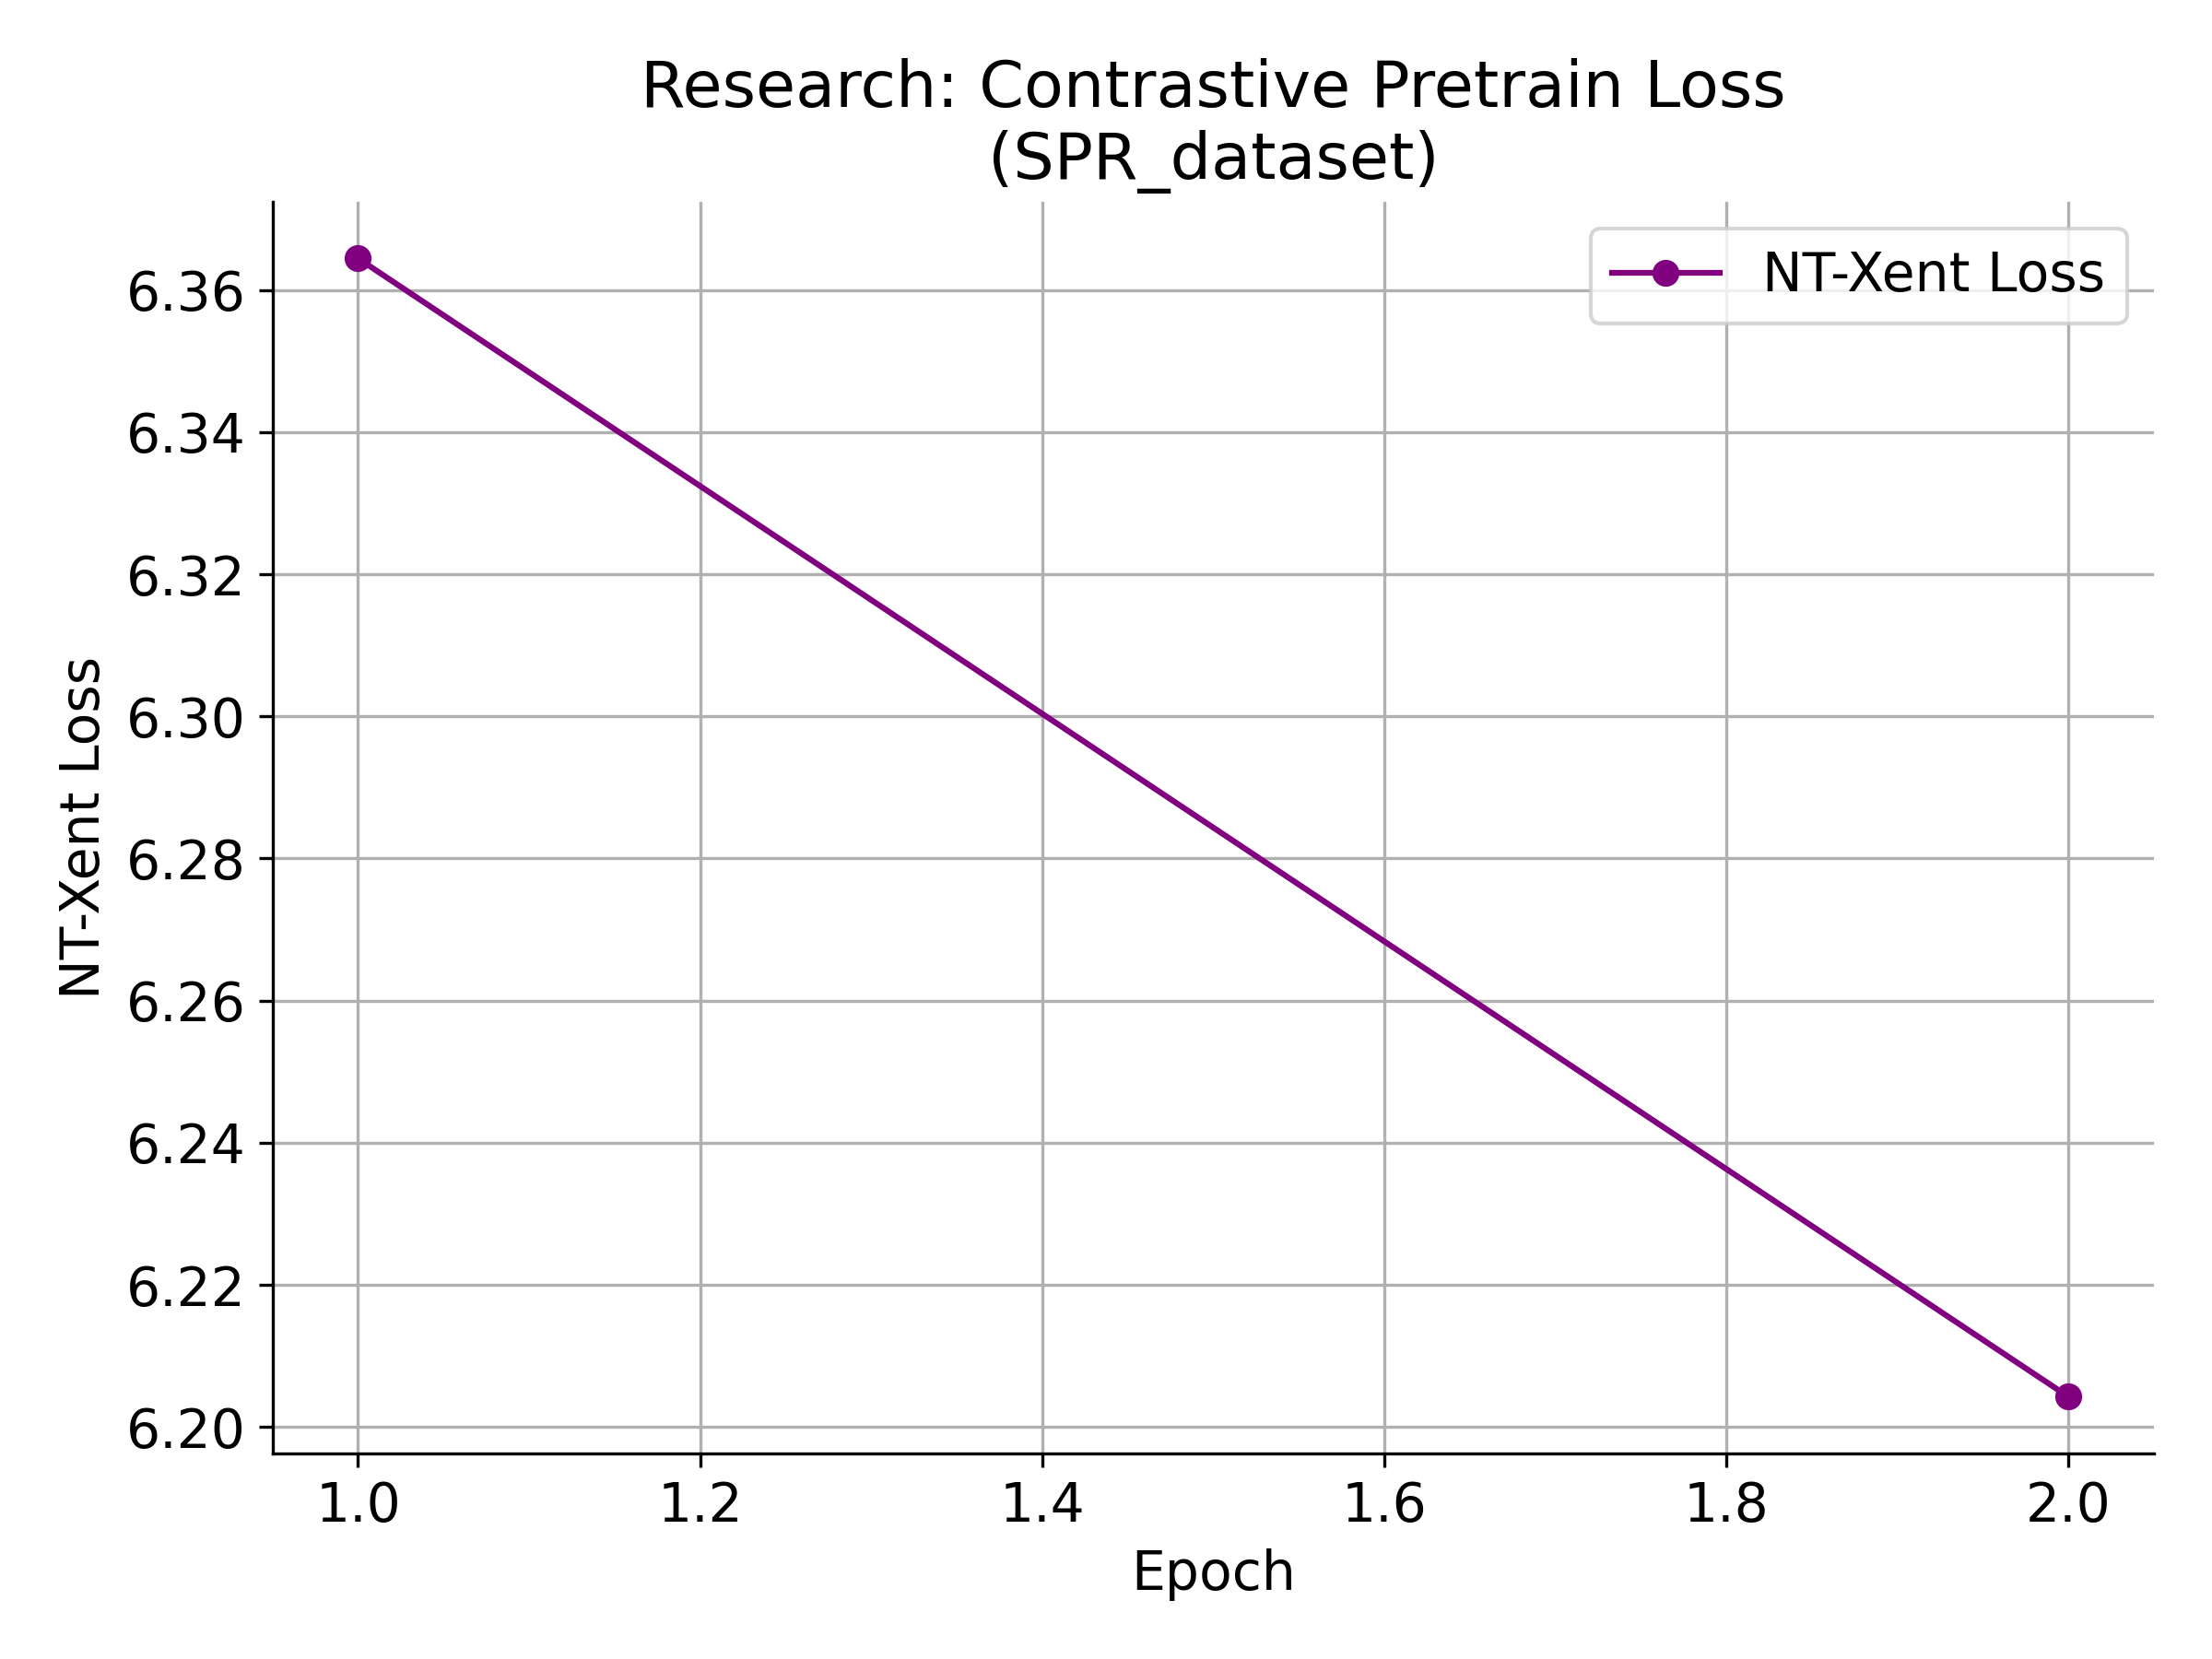
\includegraphics[width=0.49\linewidth]{research_contrastive_loss.png}
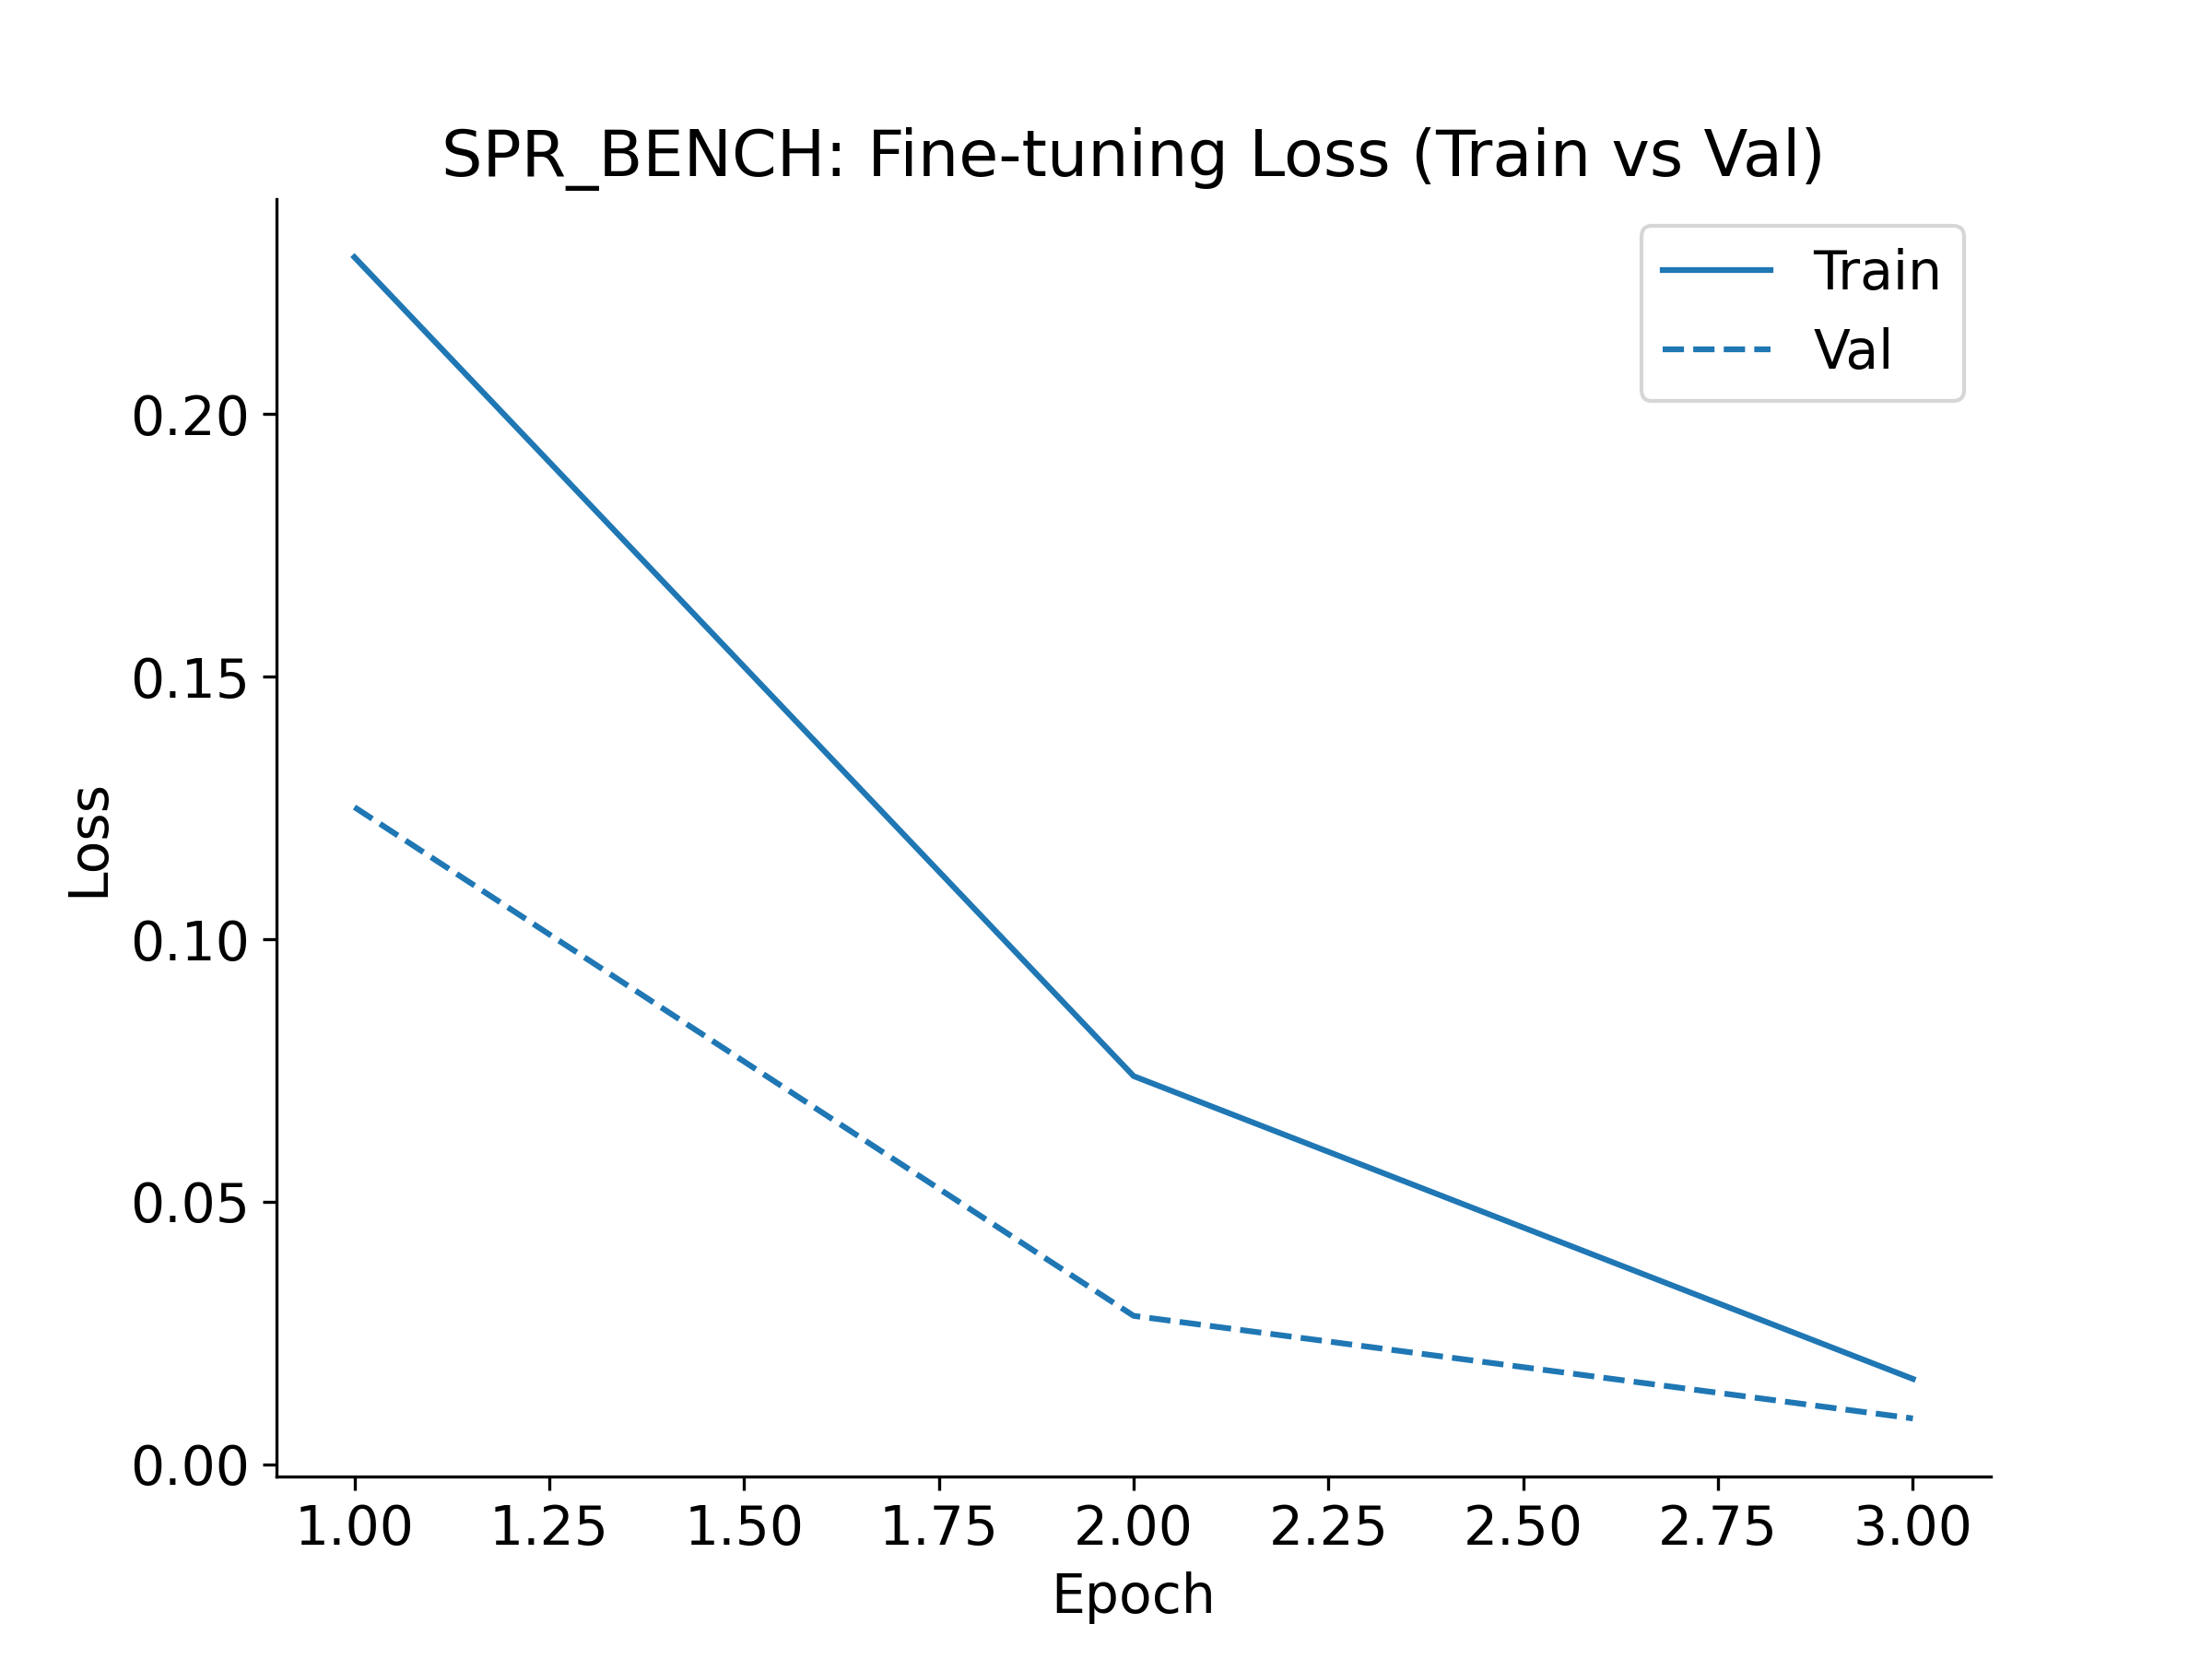
\includegraphics[width=0.49\linewidth]{research_finetune_loss.png}
\caption{Training curves for contrastive (left) and fine-tuning cross-entropy (right) losses. Notice partial improvements followed by plateaus, hinting at representational bottlenecks.}
\label{fig:main_training}
\end{figure}

To explore ablations, we selectively disabled components (e.g., projector, certain augmentations). In Figure~\ref{fig:ablation_main}, we display the three most critical ablation conditions. Each reveals substantial drops in final accuracy, suggesting that domain-specific constraints are crucial.

\begin{figure}[t]
\centering
\includegraphics[width=0.32\linewidth]{ablation_no_projector.png}
\includegraphics[width=0.32\linewidth]{ablation_no_pretrain.png}
\includegraphics[width=0.32\linewidth]{ablation_no_encodergrad.png}
\caption{Ablation results: removing projector, removing pretraining, or freezing encoder each degrades performance notably.}
\label{fig:ablation_main}
\end{figure}

\section{Conclusion}
Our study shows that contrastive pretraining can yield partial gains but also exposes pitfalls when dealing with symbolic tasks. Lessons learned include the importance of domain-specific constraints and robust projector design. Future work could address stability and injector modules that better preserve structural consistency.

\bibliography{references}

\clearpage
\appendix

\section{Additional Figures}
\begin{figure}[h]
\centering
\includegraphics[width=0.32\linewidth]{detail_cowa_baseline.png}
\includegraphics[width=0.32\linewidth]{detail_cowa_epoch.png}
\includegraphics[width=0.32\linewidth]{detail_contrastive_metrics.png}
\caption{Additional metrics and baseline comparisons.}
\label{fig:appendix_figure1}
\end{figure}

\end{document}